\scanpage{21}
\mspage{8}

% top left, four lines
\[
\begin{aligned}
&x^2+y^2+z^2+2yz+2zx-2xy=\\
&\deleted{{\unsure{\xi|\zeta}}^2+\eta^2+2(\xi+\eta)}+\\
&\xi^2+\eta^2-2\xi\eta+2(\xi+\eta)+1\\
&(\underbrace{\xi-\eta}_{\unsure{u|U}})^2+2(\underbrace{\xi+\eta}_{\unsure{v|V}})+1
\end{aligned}
\]

% upper left, below sloping rule
\figure{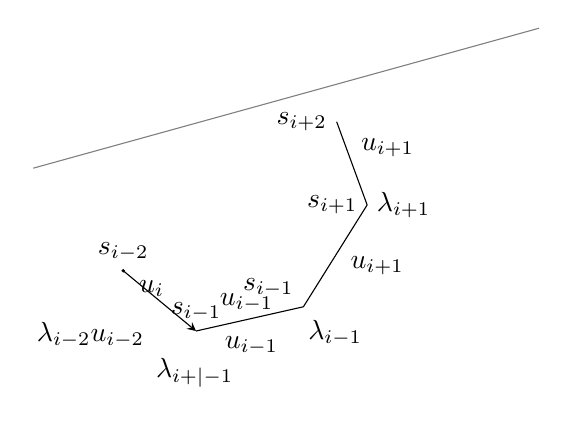
\begin{tikzpicture}[scale=.88,>=stealth]
\draw[gray,thin] (-1.3,2.48)--(6,4.5);
\coordinate (a) at (0,1.0); \coordinate (b) at (1.05,.13); \coordinate (c) at (2.6,.48); \coordinate (d) at (3.52,1.95); \coordinate (e) at (3.08,3.15);
\fill (a) circle (.8pt); \draw[->] (a)--(b); \draw (b)--(c) (c)--(d) (d)--(e);
\node[above] at (a) {$s_{i-2}$}; \node[above] at (b) {$s_{i-1}$};
\node[above left] at (c) {$s_{i\deleted{\unsure{-1}}}$};
\node[left] at (d) {$s_{i+1}$}; \node[left] at (e) {$s_{i+2}$};
\node at (.41,.74) {$\deleted{\unsure{u_{i}}}$};
\node[below left] at (.44,.4) {$\lambda_{i-2}u_{i-2}$};
\node[above] at (1.78,.26) {$\deleted{\unsure{u_{i-1}}}$}; \node[below] at (1.85,.19) {$u_{i-1}$};
\node[below] at (1.03,-.12) {$\lambda_{i\unsure{+|-}1}$};
\node[below right] at (2.53,.43) {$\lambda_{i\deleted{\unsure{-1}}}$};
\node[right] at (3.14,1.07) {$u_{i\deleted{\unsure{+1}}}$}; \node[right] at (d) {$\lambda_{i+1}$};
\node[right] at (3.29,2.77) {$u_{i+1}$};
\end{tikzpicture}}

% above boxed recurrence
\[
\deleted{\lambda_{i+1}u_i-\lambda_{i+2}(u_{i+1}+u_{i+2})+\lambda_{i+3}u_{i+3}}=0
\]

% middle, boxed
\[
\boxed{\lambda_{i-1}u_{i-2}-\lambda_i(u_{i-1}+u_i)+\lambda_{i+1}u_{i+1}=0}
\]

% middle left
\figure{\begin{tikzpicture}[scale=.83,>=stealth]
\draw[->] (0,0)--(1.45,-.04) node[midway,below] {$u_0$};
\node[below left] at (0,0) {$s_0$}; \draw[->] (1.56,.03)--(2.18,1.33) node[midway,right] {$u_1$};
\draw[->] (2.14,1.49)--(1.77,2.60) node[midway,right] {$u_2$};
\node at (.16,2.25) {$\deleted{\unsure{x}}$};
\end{tikzpicture}}

% middle right
\[
\underbrace{u_0\quad u_1}_{\text{base}}\qquad u_2=\unsure{\xi|x}u_0+\unsure{y|\eta}u_1
\]

% middle right, expressions for u₃,u₄,u₅
\[
\begin{aligned}
u_3&=\frac1{\lambda_3}\big(\lambda_2(u_1+u_2)-\lambda_1u_0\big)\\
u_4&=\frac1{\lambda_3\lambda_4}\big(\hspace{4em}-\\
u_5&=\frac1{\lambda_3\lambda_4\lambda_5}\big(\quad\rule{5em}{.35pt}\quad\big)
\end{aligned}
\]

% lower left beside u₅
\figure{\begin{tikzpicture}[scale=.75,>=stealth]
\draw[->] (0,.75)--(.86,.06); \draw[->] (.92,0)--(1.72,0); \draw (1.72,0)--(1.96,0); \fill (1.96,0) circle (2pt);
\draw[->] (2.08,0)--(3.05,0); \draw[->] (3.12,.12)--(3.68,1.12);
\end{tikzpicture}}

% lower left, above last polygon
\figure{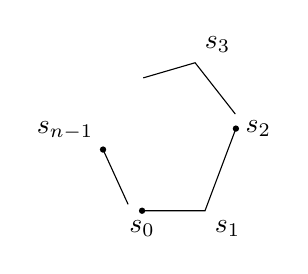
\begin{tikzpicture}[scale=.74]
\draw (0,1.05)--(.43,.11) (.67,0)--(1.75,0)--(2.28,1.41)
 (2.27,1.66)--(1.58,2.54)--(.69,2.28);
\foreach \p in {(0,1.05),(.67,0),(2.28,1.41)}{\fill \p circle (1.55pt);}
\node[above left] at (0,1.05) {$s_{n-1}$}; \node[below] at (.67,0) {$s_0$};
\node[below right] at (1.75,0) {$s_1$}; \node[right] at (2.28,1.41) {$s_2$}; \node[above right] at (1.58,2.54) {$s_3$};
\end{tikzpicture}}

% lower right, two lines
\[
\begin{aligned}
u_{n-1}&=\frac{\lambda_{n-2}}{\lambda_3\,\text{--}\,\lambda_{n-1}}
 \left(P_{n-1}u_0+\unsure{Q|B}_{n-1}u_1+R_{n-1}u_2\right)\\
u_i&=\frac{1}{\lambda_3\lambda_{\unsure{4|5}}\lambda_i}
 P_i(\lambda_1-\lambda_{i-1})u_0+\unsure{Q_i|b_i}\,\lambda_1-
\end{aligned}
\]

% foot left
\figure{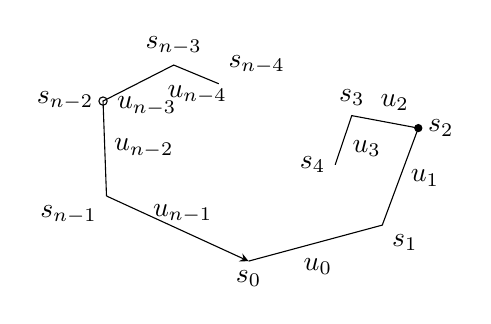
\begin{tikzpicture}[scale=.88,>=stealth]
\coordinate (a) at (2.27,0); \coordinate (b) at (4.20,.52); \coordinate (c) at (4.72,1.92);
\coordinate (d) at (3.76,2.10); \coordinate (e) at (3.52,1.39); \coordinate (f) at (1.84,2.56);
\coordinate (g) at (1.19,2.83); \coordinate (h) at (.17,2.31); \coordinate (j) at (.22,.94);
\draw (a)--(b)--(c)--(d)--(e) (f)--(g)--(h)--(j); \draw[->] (j)--(a);
\fill (c) circle (1.7pt); \draw (h) circle (1.7pt);
\foreach \p/\lbl/\pos in {a/0/below,b/1/below right,c/2/right,d/3/above,e/4/left,f/{n-4}/above right,g/{n-3}/above,h/{n-2}/left,j/{n-1}/below left}
 {\node[\pos] at (\p) {$s_{\lbl}$};}
\node[below] at (3.27,.18) {$u_0$}; \node[right] at (4.47,1.20) {$u_1$}; \node[above] at (4.38,2.03) {$u_2$};
\node[right] at (3.63,1.63) {$u_3$}; \node[below] at (1.53,2.67) {$u_{n-4}$};
\node[below] at (.80,2.51) {$u_{n-3}$}; \node[right] at (.19,1.63) {$u_{n-2}$}; \node[above] at (1.32,.41) {$u_{n-1}$};
\end{tikzpicture}}

% archive sheet number: 27
